\documentclass[a4paper,11pt]{article}

\usepackage{graphicx}
\usepackage{fullpage}
%opening
\title{Calculating persistence length}
\author{Petr \v{S}ulc}

\begin{document}

\maketitle
This example shows how to calculate a persistence length of a duplex DNA. Compile the code and copy it to the PERSISTENCE\_LENGTH directory.
Then you need to run 

\begin{verbatim}
 oxDNA input_persistence
\end{verbatim}

Note that for caclulation of persistence length, one needs a large number of decorrelated states. The program will produce a trajectory.dat file. To analyze the data, use the python script 
dspl.py:
\begin{verbatim}
 dspl.py trajectory.dat init.top 10 50
\end{verbatim}
This program will produce a table of correlations between helical vectors , $\langle {\bf n_k} \cdot {\bf n_0} \rangle$. The persistence length can be obtained from the following equation:
\begin{equation}
\langle {\bf n_k} \cdot {\bf n_0} \rangle = \exp(- k \langle l_0 \rangle /L_{ps}).
\label{exp_decay}
\end{equation}


\begin{figure}
\centering
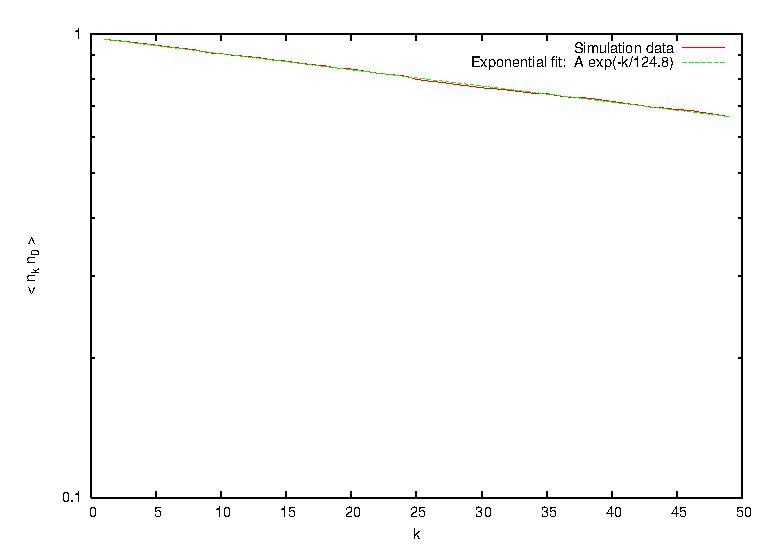
\includegraphics[width=0.9\textwidth]{ds}
\caption{The figure shows an example of an exponential fit to the data obtained from the simulation. In this case, the data show persistence length of 124 base pairs.}
\label{fig_fray}
\end{figure}


\end{document}
